\usepackage{figures/tikzit}
\usepackage{graphicx}
\usepackage[inkscapelatex=false]{svg}
\usepackage{amssymb}
\usepackage{xparse}
\usepackage{stmaryrd}
\usepackage{tikz-cd}
\usepackage{mathtools}

\newcommand{\svg}[3]{\raisebox{#1em}{\scalebox{#2}{\includesvg{imgs/#3}}}}

\newcommand{\await}{\iftoggle{static}{}{\pause}}

\tikzset{
    invisible/.style={opacity=0},
    visible on/.style={alt={#1{}{invisible}}},
    alt/.code args={<#1>#2#3}{%
        \alt<#1>{\pgfkeysalso{#2}}{\pgfkeysalso{#3}}%
    }
}

\input{macros/sets}
\input{macros/category}
\input{macros/circuits}
\input{macros/streams}

\input{figures/circuits.tikzdefs}
\input{figures/circuits.tikzstyles}

\definecolor{back}{HTML}{f8f8f2}
\newcommand{\bgcolour}{back}

\graphicspath{{./imgs/}}

\usetheme[
  background=light,
  numbering=counter,
  block=fill,
  sectionpage=none
]{metropolis}

% FiraFonts
\usepackage[sfdefault]{FiraSans}
\usepackage{FiraMono}
% Use thinner fonts
\makeatletter
\def\bfseries@sf{medium}
\def\mdseries@sf{l}
\makeatother

\definecolor{backg}{RGB}{9,72,61}
\definecolor{accent}{RGB}{0,150,136}

\definecolor{dracback}{RGB}{40, 42, 54}
\definecolor{dracfore}{RGB}{248, 248, 242}
\definecolor{dractitle}{RGB}{56, 58, 89}
\definecolor{dracblock}{RGB}{98, 114, 164}
\definecolor{draccent}{RGB}{255, 121, 198}

\setbeamercolor{normal text}{bg=dracfore}
\setbeamercolor{frametitle}{bg=dractitle, fg=dracfore}
\setbeamercolor{title separator}{fg=draccent}
\setbeamercolor{progress bar}{fg=draccent, bg=draccent}
\setbeamercolor{block title}{fg=dracfore, bg=dracblock}
\setbeamercolor{alerted text}{fg=draccent}

\newtheorem{axiom}{Axiom(s)}

\title{
    \texorpdfstring{
        \LARGE{A Fully Compositional Theory of Digital Circuits}
    }{
        A Fully Compositional Theory of Digital Circuits
    }
}
\author{
    \texorpdfstring{
        \Large\textbf{George Kaye} \\[0.25em]
        \normalsize University of Birmingham
    }{
        George Kaye
    }
}
\date{
    \texorpdfstring{
        21 June 2024 \\[0.25em]
        Applied Category Theory 2024 (ACT 2024)
    }{
        21 June 2024
    }
}

\begin{document}
\maketitle
% !TeX root = ../main-presentation.tex
\begin{frame}
    \frametitle{What are we going to be talking about?}
    \await
    \centering
    \LARGE
    Digital circuits!

    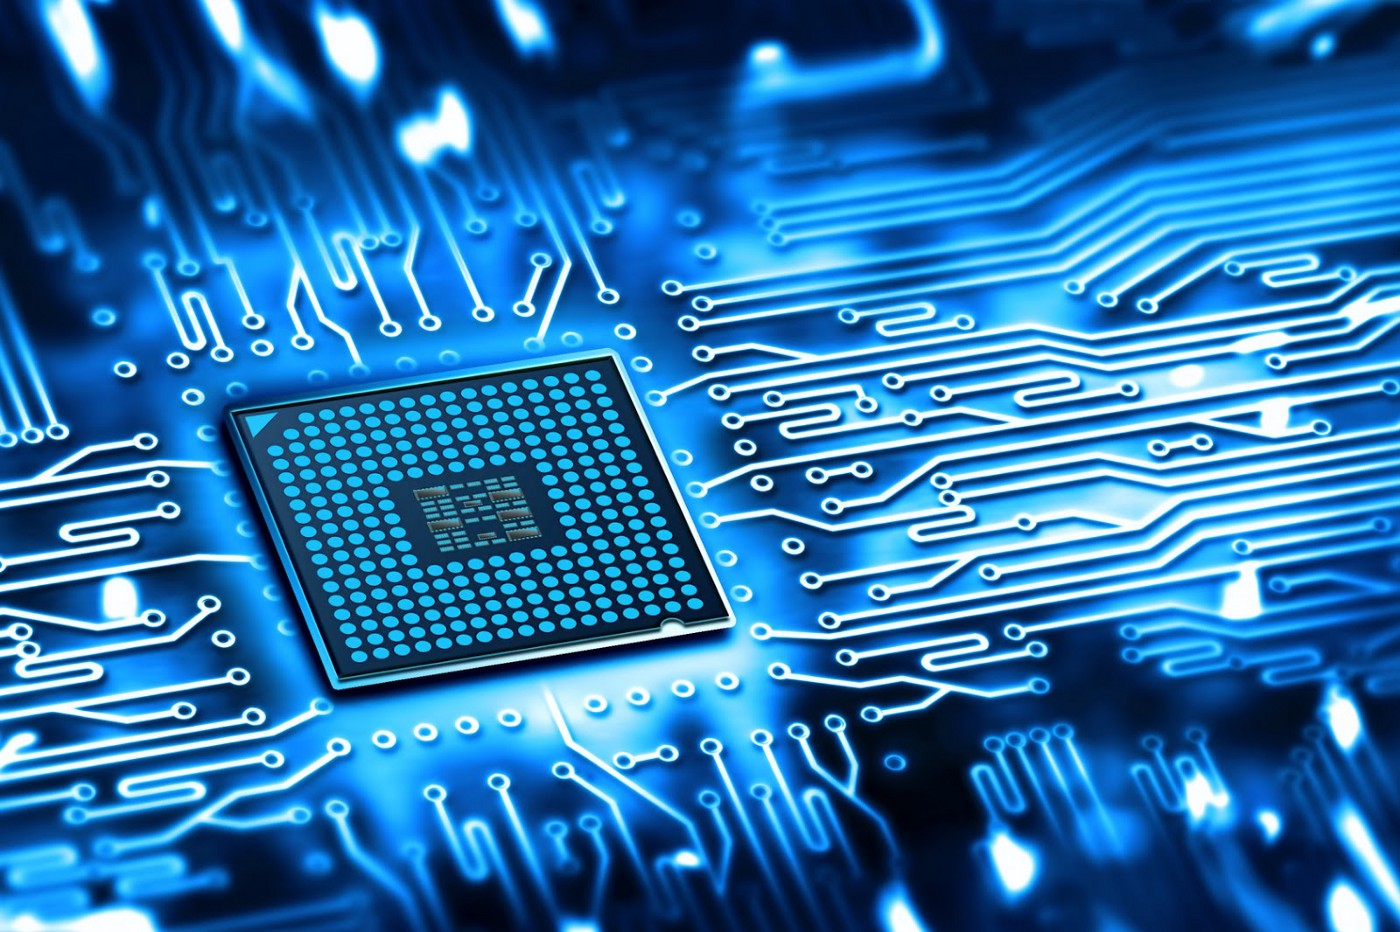
\includegraphics[width=0.6\textwidth]{imgs/circuit}
\end{frame}
\begin{frame}
    \frametitle{What are we going to be talking about?}
    \centering
    \LARGE
    Digital circuits!

    \vspace{1em}
    \normalsize

    \scalebox{2}{\tikzfig{circuits/examples/sr-latch/real-circuit}}
\end{frame}
\begin{frame}
    \frametitle{What are we going to be talking about?}

    \centering
    \Large
    We want a \alert{compositional} theory of digital circuits.

    \vspace{1em}

    \normalsize

    \await
    \dsptikzfig{strings/category/f}[box=f,colour=seq]
    \await
    \quad
    \dsptikzfig{strings/category/f}[box=g,colour=seq]
    \await
    \quad
    \dsptikzfig{strings/category/f-2-2}[box=h,colour=seq]

    \await
    \vspace{1em}

    \dsptikzfig{strings/category/composition}[box1=f,box2=g,colour=seq]
    \quad
    \dsptikzfig{strings/monoidal/tensor}[box1=f,box2=g,colour=seq]
    \quad
    \dsptikzfig{strings/traced/trace-rhs}[box=h,colour=seq]

    \await

    \Large
    \vspace{1em}

    Using \alert{string diagrams} removes \\ much of the bureacracy

    \await

    \normalsize

    (also they look pretty)

\end{frame}

\begin{frame}
    \frametitle{The story so far}

    \centering
    \LARGE

    How did we get here?

    
\includegraphics[width=0.5\textwidth]{imgs/megabus}

\end{frame}

\begin{frame}
    \frametitle{The story so far}

    \centering

    \scalebox{8}{\textbf{2003}}

\end{frame}

\begin{frame}
    \frametitle{The story so far}

    \centering
    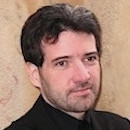
\includegraphics[width=0.3\textwidth]{imgs/lafont}

    \LARGE
    \textbf{Yves Lafont}

    \normalsize
    \emph{`Towards an algebraic theory of Boolean circuits'}

\end{frame}

\begin{frame}
    \frametitle{The story so far}

    \centering

    \scalebox{8}{\textbf{2016}}

\end{frame}

\begin{frame}
    \frametitle{The story so far}

    \centering

    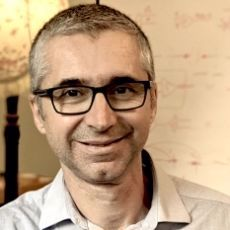
\includegraphics[width=0.25\textwidth]{imgs/ghica}
    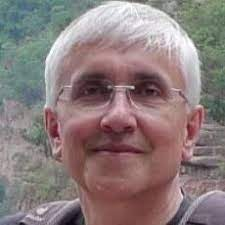
\includegraphics[width=0.25\textwidth]{imgs/achim}
    
\includegraphics[width=0.25\textwidth]{imgs/lopez}

    \LARGE
    \textbf{Dan Ghica, Achim Jung, Aliaume Lopez}

    \normalsize
    \emph{`Diagrammatic semantics for digital circuits'}


\end{frame}

\begin{frame}
    \frametitle{The story so far}

    \centering

    \scalebox{8}{\textbf{2019}}

\end{frame}

\begin{frame}
    \frametitle{The story so far}

    \centering

    \begin{minipage}{0.45\textwidth}
        \centering

        \phantom{\textbf{David Sprunger}}

        \vspace{0.5em}

        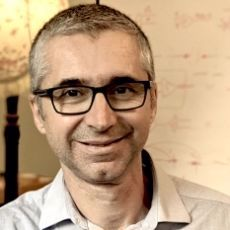
\includegraphics[width=8em]{imgs/ghica}

        \visible<\iftoggle{static}{1}{2-}>{\emph{`Do you know category theory'}}

        \visible<\iftoggle{static}{1}{4-}>{\emph{`Do you want to do circuits stuff'}}
    \end{minipage}
    \begin{minipage}{0.25\textwidth}
        \centering

        \phantom{\textbf{David Sprunger}}

        \vspace{0.5em}

        
\includegraphics[width=8em]{imgs/kaye}%

        \visible<\iftoggle{static}{1}{3-}>{\emph{`No'}}

        \visible<\iftoggle{static}{1}{5-}>{\emph{`Okay'}}
    \end{minipage}
    \visible<\iftoggle{static}{1}{6-}>{%
        \begin{minipage}{0.25\textwidth}
            \centering

            \textbf{David Sprunger}

            \vspace{0.5em}

            
\includegraphics[width=8em]{imgs/sprunger}

            \phantom{hello}

            \emph{`I will help too'}
        \end{minipage}%
    }
\end{frame}
\section{Syntax}

\begin{frame}
    \frametitle{Put the pieces together}

    \centering
    \scalebox{4}{\textbf{Syntax}}

\end{frame}

\begin{frame}
    \frametitle{Combinational circuit components}
    \centering
    \await

    \vspace{-0.5em}

    \renewcommand{\arraystretch}{2}
    \begin{tabular}{cccccc}
        \multicolumn{2}{c}{\visible<2->{\alert{gates}}}
                                                                                    &
        \multicolumn{2}{c}{\visible<3->{\alert{(co)monoid structure}}}              &

        \multicolumn{2}{c}{\visible<3->{\alert{categorical structure}}}
        \\
        \visible<2->{\dsptikzfig{circuits/components/gates/and}}                    &
        \visible<2->{AND gate}                                                      &
        \hspace{0.175cm}
        \visible<3->{\dsptikzfig{strings/structure/monoid/init}[colour=comb]}       &
        \visible<3->{introduce}                                                     &
        \visible<3->{\dsptikzfig{strings/category/identity}[colour=comb]}           &
        \visible<3->{identity}                                                        \\
        \visible<2->{\dsptikzfig{circuits/components/gates/or}}                     &
        \visible<2->{OR gate}                                                       &
        \visible<3->{\,\,\dsptikzfig{strings/structure/comonoid/copy}[colour=comb]} &
        \visible<3->{fork}                                                          &
        \visible<3->{\dsptikzfig{strings/symmetric/symmetry}[colour=comb]}          &
        \visible<3->{symmetry}                                                        \\
        \visible<2->{\dsptikzfig{circuits/components/gates/not}}                    &
        \visible<2->{NOT gate}                                                      &
        \visible<3->{\,\,\dsptikzfig{strings/structure/monoid/merge}[colour=comb]}  &
        \visible<3->{join}                                                            \\
                                                                                    &
                                                                                    &
        \,\,\,\,
        \visible<3->{\dsptikzfig{strings/structure/comonoid/discard}[colour=comb]}
        \hspace{0.175cm}                                                            &
        \visible<3->{eliminate}                                                     &
    \end{tabular}

    \vspace{0.5em}

    \await
    \alert{Light} circuits \(
    \dsptikzfig{strings/category/f}[box=f,colour=comb]
    \) only contain gates and structure.

    \scriptsize
    \await
    (actually, we do it more generally than this, but let's keep it simple)
\end{frame}
\begin{frame}
    \frametitle{Sequential circuit components}

    \renewcommand{\arraystretch}{1.75}

    \await

    \begin{minipage}{0.3\textwidth}
        \centering
        \alert{Values}

        \begin{tabular}{rl}
            \dsptikzfig{circuits/components/values/vs}[val=\belnapfalse] &
            false                                                          \\
            \dsptikzfig{circuits/components/values/vs}[val=\belnaptrue]  &
            true                                                           \\
            \await
            \dsptikzfig{circuits/components/values/vs}[val=\top]         &
            short circuit
        \end{tabular}

        \vspace{1em}

        \dsptikzfig{circuits/a4}

    \end{minipage}
    \await
    \qquad
    \begin{minipage}{0.6\textwidth}
        \centering
        \begin{tabular}{cc}
            \alert{Delay} &
            \alert{Feedback} \\
            \(
            \dsptikzfig{circuits/components/waveforms/delay}
            \)
                          &

            \(
            \dsptikzfig{strings/category/f-2-2}[box=f,colour=seq]
            \,\,\Rightarrow\,\,
            \dsptikzfig{strings/traced/trace-rhs}[box=f,colour=seq]
            \)
        \end{tabular}

        \vspace{2em}

        \visible<3->{
            \alert{Dark} circuits \(
            \dsptikzfig{strings/category/f}[box=f,colour=seq]
            \) may contain \\[1em] delay or feedback.
        }

    \end{minipage}

\end{frame}
\begin{frame}
    \frametitle{Building circuits}

    \centering
    \LARGE
    Circuits are morphisms in a
    \alert{freely generated symmetric traced monoidal category} (STMC).

    \vspace{1em}

    \await
    \dsptikzfig{strings/category/composition}[box1=f,box2=g,colour=seq]
    \await
    \quad
    \dsptikzfig{strings/monoidal/tensor}[box1=f,box2=g,colour=seq]
    \await
    \quad
    \dsptikzfig{strings/traced/trace-rhs}[box=f,colour=seq]

\end{frame}

\begin{frame}
    \frametitle{Breaking the mould}

    \centering
    \LARGE

    Why not use \alert{Frobenius} structure?

    \normalsize

    \vspace{0.5em}

    \iltikzfig{strings/traced/trace-from-product}[colour=seq]

    \vspace{1em}

    \LARGE
    We want \alert{copying}...

    \pause
    \normalsize

    \vspace{1em}

    \iltikzfig{strings/structure/cartesian/naturality-copy-lhs}[box=f,colour=seq]
    \(=\)
    \iltikzfig{strings/structure/cartesian/naturality-copy-rhs}[box=f,colour=seq]
    \qquad
    \pause
    \iltikzfig{strings/structure/bialgebra/init-copy-lhs}
    \(=\)
    \iltikzfig{strings/structure/bialgebra/init-copy-rhs}

    \vspace{1em}
    \pause

    \iltikzfig{strings/traced/trace-from-product}[colour=seq]
    \(=\)
    \iltikzfig{strings/traced/trace-from-product-1}[colour=seq]

\end{frame}
\section{Previous work}

\begin{frame}
    \frametitle{Where were we?}

    \centering
    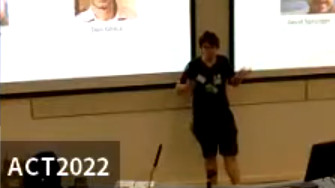
\includegraphics[width=0.75\textwidth]{imgs/act2022}

\end{frame}

\begin{frame}
    \frametitle{What is the meaning?}

    \centering
    \Large

    What are the \alert{denotational semantics} of digital circuits?

    \await

    Certain kinds of \alert{stream functions}!
    \[
        f(v_0 \streamcons v_1 \streamcons v_2 \streamcons \dots)
        =
        w_0 \streamcons w_1 \streamcons w_2 \streamcons \dots
    \]

    \await

    \LARGE

    \alert{Denotational} equivalence
    \[\circuittostream[\iltikzfig{strings/category/f}[colour=seq]]{}
        =
        \circuittostream[\iltikzfig{strings/category/f}[box=g,colour=seq]]{}
        \Rightarrow
        \iltikzfig{strings/category/f}[colour=seq]
        \approx
        \iltikzfig{strings/category/f}[box=g,colour=seq]
    \]
\end{frame}
\begin{frame}
    \frametitle{Guards, guards!}

    \centering
    \Large

    We can also \alert{eliminate non-delay-guarded feedback}
    \[
        \dsptikzfig{strings/traced/trace-rhs}[colour=comb]
        \approx
        \dsptikzfig{circuits/instant-feedback/general}
    \]

    (Kleene fixpoint theorem)

\end{frame}
\begin{frame}
    \frametitle{We want something different}

    \centering
    \Large

    Denotational equivalence obscures the \alert{structure} of terms

    \await

    We want to reason more \alert{syntactically}

    \vspace{1em}

    \LARGE
    \begin{minipage}{0.45\textwidth}
        \centering
        Operational
        semantics

        \large
        a bit has changed
    \end{minipage}
    \begin{minipage}{0.45\textwidth}
        \centering
        Algebraic
        semantics

        \large
        (pretty much) new
    \end{minipage}
\end{frame}
% !TeX root = ../main-presentation.tex
\section{Operational semantics}

\begin{frame}
    \frametitle{Doing something useful}

    \centering

    \LARGE
    Suppose we have two circuits \\
    with the same denotation
    \normalsize

    \vspace{2em}

    \(
    \left\llbracket\dsptikzfig{strings/category/f}[box=f,colour=seq]\right\rrbracket
    =
    \left\llbracket\dsptikzfig{strings/category/f}[box=g,colour=seq]\right\rrbracket
    \)

    \vspace{2em}

    \LARGE
    \await
    What does this tell us about the \\
    \alert{structure} of these circuits?

\end{frame}
\begin{frame}
    \frametitle{Reducing it down}

    \await

    \centering
    \scalebox{4}{\textbf{Operational}}

    \scalebox{4}{\textbf{semantics}}

\end{frame}
\begin{frame}
    \frametitle{Reducing it down}

    \centering
    \LARGE

    We want to find a set of \\ \alert{reductions} for digital circuits


    \await
    We want to reduce circuits to their outputs \alert{syntactically}
    in a \alert{step-by-step} manner

\end{frame}
\begin{frame}
    \frametitle{Going global}

    \centering

    \dsptikzfig{strings/category/f}[box=f,colour=seq]
    \await
    \Large=\normalsize
    \dsptikzfig{circuits/productivity/trace-delay}[core=\hat{f},state=\listvar{v}]

    \vspace{1em}
    \Large
    by moving boxes and wires around
\end{frame}

\begin{frame}
    \frametitle{Going global}

    \centering
    \Large

    \await

    \normalsize
    \begin{gather*}
        \dsptikzfig{circuits/components/waveforms/register}
        \coloneqq
        \dsptikzfig{circuits/components/waveforms/register-shorthand}
        \qquad
        \Large
        \text{\alert{`Register'}}
    \end{gather*}

    \vspace{1em}

    \await

    \dsptikzfig{circuits/productivity/trace-delay}[core=f,state=\listvar{v}]
    \Large\(\reduction\)\normalsize
    \dsptikzfig{circuits/productivity/mealy-rule}[core=\hat{f}]

    \await

    \dsptikzfig{strings/category/f}[box=f,colour=seq]
    \Large\(\reductions\)\normalsize
    \dsptikzfig{circuits/productivity/pre-mealy-form}[core=\hat{f},state=\listvar{s}]
    \Large\(\reductions\)\normalsize
    \dsptikzfig{circuits/productivity/mealy-form}[core=\tilde{f},state=\overline{s}]

\end{frame}
\begin{frame}
    \frametitle{What is the goal}

    \centering

    \await
    \Large
    We want to compute the \alert{outputs} of circuits given some \alert{inputs}
    \normalsize

    \begin{gather*}
        \dsptikzfig{circuits/productivity/productive-goal-lhs}[box=f]
        \reductions
        \dsptikzfig{circuits/productivity/productive-goal-rhs}[box=g]
    \end{gather*}

    \await

    \vspace{1em}

    \Large

    How does a circuit \alert{process} a value?

\end{frame}
\begin{frame}
    \frametitle{Reducing values}

    \begin{gather*}
        \dsptikzfig{circuits/axioms/gate-lhs}
        \reduction
        \dsptikzfig{circuits/axioms/gate-rhs}
        \qquad
        \dsptikzfig{circuits/axioms/fork-lhs}
        \reduction
        \dsptikzfig{circuits/axioms/fork-rhs}
        \\[0.5em]
        \dsptikzfig{circuits/axioms/join-lhs}
        \reduction
        \dsptikzfig{circuits/axioms/join-rhs}
        \qquad
        \dsptikzfig{circuits/axioms/stub-lhs}
        \reduction
        \dsptikzfig{strings/monoidal/empty}
    \end{gather*}

    \await
    \vspace{1em}
    \Large

    \begin{lemma}
        For every
        \dsptikzfig{strings/category/f}[box=f,colour=comb]
        there exists
        \dsptikzfig{circuits/components/values/vs}[val=\listvar{w}]
        s.t.
        \dsptikzfig{circuits/components/circuits/f-applied}[box=f,colour=comb]
        \(\reductions\)
        \dsptikzfig{circuits/components/values/vs}[val=\listvar{w}].
    \end{lemma}

\end{frame}


\begin{frame}
    \frametitle{Catching the jet stream}

    \Large

    What about \alert{delays}?

    \normalsize

    \begin{gather*}
        \visible<\iftoggle{static}{1}{2-}>{\dsptikzfig{circuits/axioms/generalised-streaming-lhs}[box=f]}
        \visible<\iftoggle{static}{1}{3-}>{\coloneqq}
        \visible<\iftoggle{static}{1}{3-}>{\dsptikzfig{circuits/axioms/generalised-streaming-lhs-verbose}[box=f]}
        \visible<\iftoggle{static}{1}{4-}>{\reduction}
        \visible<\iftoggle{static}{1}{4-}>{\dsptikzfig{circuits/axioms/generalised-streaming-rhs}[box=f]}
        \qquad
        \visible<\iftoggle{static}{1}{5-}>{\text{\alert{'Streaming'}}}
    \end{gather*}
\end{frame}

\begin{frame}
    \frametitle{Catching the jet stream}

    \vspace{-2em}

    \begin{gather*}
        \visible<\iftoggle{static}{1}{2-}>{\dsptikzfig{circuits/productivity/productive-goal-lhs}[box=f]}
        \visible<\iftoggle{static}{1}{3-}>{\reduction}
        \visible<\iftoggle{static}{1}{3-}>{\dsptikzfig{circuits/productivity/mealy-form-applied}[core=\hat{f}]}
        \visible<\iftoggle{static}{1}{4-}>{\reduction}
        \visible<\iftoggle{static}{1}{4-}>{\dsptikzfig{circuits/productivity/mealy-form-streamed}[core=\hat{f}]}
        \\[0.75em]
        \visible<\iftoggle{static}{1}{5-}>{\reduction}
        \visible<\iftoggle{static}{1}{5-}>{\dsptikzfig{circuits/productivity/mealy-form-instant}[core=\hat{f}]}
        \visible<\iftoggle{static}{1}{6-}>{\reduction}
        \visible<\iftoggle{static}{1}{6-}>{\dsptikzfig{circuits/productivity/mealy-form-instant-registers}[core=\hat{f}]}
        \\[0.75em]
        \visible<\iftoggle{static}{1}{7-}>{\reduction}
        \visible<\iftoggle{static}{1}{7-}>{\dsptikzfig{circuits/productivity/mealy-form-produced}[core=\hat{f}]}
        \visible<\iftoggle{static}{1}{8-}>{\coloneqq}
        \visible<\iftoggle{static}{1}{8-}>{\dsptikzfig{circuits/productivity/productive-goal-rhs}[box=g]}
    \end{gather*}
\end{frame}

\begin{frame}
    \frametitle{Observe this}

    \centering
    \LARGE

    When are two circuits \alert{observationally equivalent}?

    \await

    Circuits have \alert{finitely many states}...

    \vspace{1em}

    \dsptikzfig{circuits/productivity/mealy-form}[core=f,state=s]
    \quad
    \dsptikzfig{circuits/productivity/mealy-form}[core=f,state=t]
    \quad
    \dsptikzfig{circuits/productivity/mealy-form}[core=f,state=u]
    \quad
    \(\cdots\)

    Maximum number of states: \(|\values|^{\text{number of delays}}\)

\end{frame}
\begin{frame}
    \frametitle{Observe this}

    \centering
    \Large

    \(
    \dsptikzfig{strings/category/f}[colour=seq]
    \sim
    \dsptikzfig{strings/category/f}[colour=seq,box=g]
    \)

    \qquad

    Two circuits are \alert{observationally equivalent} if the
    reduction procedure creates the same outputs for all inputs of length
    \(|\values|^{\text{max number of delays}} + 1\).

\end{frame}

\begin{frame}
    \frametitle{Observe this}

    \centering
    \Large

    \(
    \dsptikzfig{strings/category/f}[colour=seq]
    \approx
    \dsptikzfig{strings/category/f}[colour=seq,box=g]
    \Leftrightarrow
    \dsptikzfig{strings/category/f}[colour=seq]
    \sim
    \dsptikzfig{strings/category/f}[colour=seq,box=g]
    \)

    \await

    \vspace{1em}

    \LARGE
    Denotational semantics \(\cong\) Operational semantics

\end{frame}
\section{Algebraic semantics}

\begin{frame}
    \frametitle{Still takes a while}

    \centering
    \LARGE

    This is a \alert{superexponential} upper bound for \\
    testing circuit equivalence

    \vspace{1em}
    \await
    Can we do better?

\end{frame}

\begin{frame}
    \frametitle{Mealy is so back}
    \centering

    \Large
    First things first...

    \normalsize
    \await
    \begin{gather*}
        \dsptikzfig{strings/structure/monoid/unitality-l-lhs}
        =
        \dsptikzfig{strings/structure/monoid/unitality-l-rhs}
        \quad
        \dsptikzfig{strings/structure/monoid/unitality-r-lhs}
        =
        \dsptikzfig{strings/structure/monoid/unitality-r-rhs}
        \\[0.25em]
        \rule{\textwidth}{0.1mm}
        \\[0.5em]
        \dsptikzfig{circuits/axioms/bottom-delay-lhs}
        =
        \dsptikzfig{circuits/axioms/bottom-delay-rhs}
        \quad
        \dsptikzfig{circuits/instant-feedback/equation-lhs}
        =
        \dsptikzfig{circuits/instant-feedback/fixpoint-concrete}
    \end{gather*}

    \Large
    By these equations, \(
    \dsptikzfig{strings/category/f}[box=F,colour=seq]
    =
    \dsptikzfig{circuits/productivity/mealy-form}
    \)

\end{frame}
\begin{frame}
    \frametitle{It's completely normal}

    \centering
    \LARGE

    \await

    Say we have a procedure \(\lvert-\rvert\) for
    establishing a \alert{canonical circuit} for a function
    \(\morph{f}{\valuetuple{m}}{\valuetuple{n}}\)

    \await

    \vspace{1em}

    A circuit is \alert{normalised} if it is in the image of \(\lvert-\rvert\)

    \await

    \vspace{1em}

    What equations are needed to \\ normalise any circuit?

\end{frame}
\begin{frame}
    \frametitle{It's completely normal}

    \centering

    \vspace{1em}

    \begin{minipage}{0.4\textwidth}
        \centering
        \scalebox{0.6}{
            \(
            \dsptikzfig{circuits/axioms/belnap/translation/explosion-lhs}
            =
            \dsptikzfig{circuits/axioms/belnap/translation/explosion-rhs}
            \)
        }
    \end{minipage}
    \begin{minipage}{0.55\textwidth}
        \centering
        \scalebox{0.6}{
            \(
            \dsptikzfig{circuits/axioms/belnap/translation/join-and-lhs}
            =
            \dsptikzfig{circuits/axioms/belnap/translation/join-and-rhs}
            \)
            \quad
            \(
            \dsptikzfig{circuits/axioms/belnap/translation/de-morgan-and-lhs}
            =
            \dsptikzfig{circuits/axioms/belnap/translation/de-morgan-and-rhs}
            \)
        }
        \\[0.25em]
        \rule{\textwidth}{0.1mm}
        \\[0.5em]
        \scalebox{0.6}{
            \(
            \dsptikzfig{circuits/axioms/belnap/translation/join-or-lhs}
            =
            \dsptikzfig{circuits/axioms/belnap/translation/join-or-rhs}
            \)
            \quad
            \(
            \dsptikzfig{circuits/axioms/belnap/translation/de-morgan-or-lhs}
            =
            \dsptikzfig{circuits/axioms/belnap/translation/de-morgan-or-rhs}
            \)
        }
    \end{minipage}
    \\[0.25em]
    \rule{\textwidth}{0.1mm}
    \\[0.5em]
    \scalebox{0.7}{
        \(\dsptikzfig{circuits/axioms/belnap/translation/not-fork-lhs}
        =
        \dsptikzfig{circuits/axioms/belnap/translation/not-fork-rhs}\)
        \quad
        \(\dsptikzfig{circuits/axioms/belnap/translation/and-fork-lhs}
        =
        \dsptikzfig{circuits/axioms/belnap/translation/and-fork-rhs}\)
        \quad
        \(\dsptikzfig{circuits/axioms/belnap/translation/or-fork-lhs}
        =
        \dsptikzfig{circuits/axioms/belnap/translation/or-fork-rhs}\)
        \quad
        \(\dsptikzfig{strings/structure/bialgebra/merge-copy-lhs}
        =
        \dsptikzfig{strings/structure/bialgebra/merge-copy-rhs}\)
    }
    \\[0.25em]
    \rule{\textwidth}{0.1mm}
    \\[0.5em]
    \scalebox{0.7}{
        \(\dsptikzfig{strings/structure/bialgebra/init-copy-lhs}
        =
        \dsptikzfig{strings/structure/bialgebra/init-copy-rhs}\)
        \quad
        \(\dsptikzfig{circuits/axioms/belnap/translation/and-and-idempotent-lhs}
        =
        \dsptikzfig{circuits/axioms/belnap/translation/and-and-idempotent-rhs}\)
        \quad
        \(\dsptikzfig{circuits/axioms/belnap/translation/or-or-idempotent-lhs}
        =
        \dsptikzfig{circuits/axioms/belnap/translation/or-or-idempotent-rhs}\)
    }
    \\[0.25em]
    \rule{\textwidth}{0.1mm}
    \\[0.5em]
    \scalebox{0.7}{
        \(\dsptikzfig{circuits/axioms/belnap/translation/bot-and-lhs}
        =
        \dsptikzfig{circuits/axioms/belnap/translation/bot-x-rhs}\)
        \quad
        \(\dsptikzfig{circuits/axioms/belnap/translation/bot-or-lhs}
        =
        \dsptikzfig{circuits/axioms/belnap/translation/bot-x-rhs}\)
        \quad
        \(\dsptikzfig{circuits/axioms/belnap/translation/bot-and-lhs}
        =
        \dsptikzfig{circuits/axioms/belnap/translation/bot-x-rhs}\)
        \quad
        \(\dsptikzfig{circuits/axioms/belnap/double-negation-lhs}
        =
        \dsptikzfig{circuits/axioms/belnap/double-negation-rhs}\)
    }
\end{frame}

\begin{frame}
    \frametitle{It's completely normal}
    \centering

    \vspace{1em}

    \scalebox{0.7}{\(
        \dsptikzfig{circuits/axioms/belnap/and-associativity-lhs}
        =
        \dsptikzfig{circuits/axioms/belnap/and-associativity-rhs}
        \quad
        \dsptikzfig{circuits/axioms/belnap/or-associativity-lhs}
        =
        \dsptikzfig{circuits/axioms/belnap/or-associativity-rhs}
        \quad
        \dsptikzfig{circuits/axioms/belnap/and-commutativity-lhs}
        =
        \dsptikzfig{circuits/axioms/belnap/and-commutativity-rhs}
        \)
    }
    \\[0.25em]
    \rule{\textwidth}{0.1mm}
    \\[0.5em]
    \scalebox{0.7}{\(
        \dsptikzfig{circuits/axioms/belnap/and-or-distributivity-lhs}
        =
        \dsptikzfig{circuits/axioms/belnap/and-or-distributivity-rhs}
        \quad
        \dsptikzfig{circuits/axioms/belnap/or-and-distributivity-lhs}
        =
        \dsptikzfig{circuits/axioms/belnap/or-and-distributivity-rhs}
        \quad
        \dsptikzfig{circuits/axioms/belnap/or-commutativity-lhs}
        =
        \dsptikzfig{circuits/axioms/belnap/or-commutativity-rhs}
        \)
    }
    \\[0.25em]
    \rule{\textwidth}{0.1mm}
    \\[0.5em]
    \scalebox{0.7}{\(
        \dsptikzfig{circuits/axioms/belnap/absorption-2-lhs}
        =
        \dsptikzfig{circuits/axioms/belnap/absorption-2-rhs}
        \quad
        \dsptikzfig{circuits/axioms/belnap/absorption-1-lhs}
        =
        \dsptikzfig{circuits/axioms/belnap/absorption-1-rhs}
        \quad
        \dsptikzfig{circuits/axioms/belnap/or-idempotent-lhs}
        =
        \dsptikzfig{circuits/axioms/belnap/or-idempotent-rhs}
        \)
    }
    \\[0.25em]
    \rule{\textwidth}{0.1mm}
    \\[0.5em]
    \scalebox{0.7}{\(
        \dsptikzfig{circuits/axioms/belnap/translation/and-fork-lhs}
        =
        \dsptikzfig{circuits/axioms/belnap/translation/and-fork-rhs}
        \quad
        \dsptikzfig{circuits/axioms/belnap/translation/or-fork-lhs}
        =
        \dsptikzfig{circuits/axioms/belnap/translation/or-fork-rhs}
        \quad
        \dsptikzfig{circuits/axioms/belnap/and-idempotent-lhs}
        =
        \dsptikzfig{circuits/axioms/belnap/and-idempotent-rhs}
        \)
    }
    \\[0.25em]
    \rule{\textwidth}{0.1mm}
    \\[0.5em]
    \scalebox{0.7}{\(
        \dsptikzfig{strings/structure/comonoid/commutativity-rhs}
        =
        \dsptikzfig{strings/structure/comonoid/commutativity-lhs}
        \quad
        \dsptikzfig{strings/structure/comonoid/associativity-lhs}
        =
        \dsptikzfig{strings/structure/comonoid/associativity-rhs}
        \quad
        \dsptikzfig{strings/structure/comonoid/unitality-l-lhs}
        =
        \dsptikzfig{strings/structure/comonoid/unitality-l-rhs}
        \)
    }
\end{frame}
\begin{frame}
    \frametitle{Changing the states}

    \centering
    \Large

    How to translate between \(
    \dsptikzfig{circuits/productivity/mealy-form}[core=|f|, colour=comb]
    \)
    and \(
    \dsptikzfig{circuits/productivity/mealy-form}[core=|g|, state=\listvar{t}, colour=comb]
    \)?

    \await

    \vspace{1em}

    First \alert{encode} one set of states into the other

    \vspace{0.5em}

    \(
    \dsptikzfig{circuits/algebraic/encoder-applied}[state=\listvar{s}]
    =
    \dsptikzfig{circuits/components/values/vs}[val=\listvar{t}]
    \qquad
    \dsptikzfig{circuits/algebraic/decoder-applied}[state=\listvar{t}]
    =
    \dsptikzfig{circuits/components/values/vs}[val=\listvar{s}]
    \)

    \vspace{1em}
    \normalsize
    (and for any future states)

\end{frame}
\begin{frame}
    \frametitle{Changing the states}

    \centering

    \vspace{1em}

    \scalebox{0.7}{\(
        \dsptikzfig{circuits/productivity/mealy-form}[core=|f|,delay=x, colour=seq]
        =
        \dsptikzfig{circuits/algebraic/state-encoding}[core=|f|,delay=x]
        \)
    }
    \\[0.25em]
    \rule{\textwidth}{0.1mm}
    \\[0.5em]
    \scalebox{0.7}{\(
        \dsptikzfig{circuits/axioms/gate-lhs}
        =
        \dsptikzfig{circuits/axioms/gate-rhs}
        \quad
        \dsptikzfig{circuits/axioms/fork-lhs}
        =
        \dsptikzfig{circuits/axioms/fork-rhs}
        \quad
        \dsptikzfig{circuits/axioms/join-lhs}
        =
        \dsptikzfig{circuits/axioms/join-rhs}
        \)
    }
    \\[0.25em]
    \rule{\textwidth}{0.1mm}
    \\[0.5em]
    \scalebox{0.7}{\(
        \dsptikzfig{circuits/axioms/stub-lhs}
        =
        \dsptikzfig{strings/monoidal/empty}
        \quad
        \dsptikzfig{circuits/axioms/delay-fork-lhs}
        =
        \dsptikzfig{circuits/axioms/delay-fork-rhs}
        \quad
        \dsptikzfig{circuits/axioms/bottom-delay-lhs}
        =
        \dsptikzfig{circuits/axioms/bottom-delay-rhs}
        \quad
        \dsptikzfig{circuits/axioms/streaming-lhs}
        =
        \dsptikzfig{circuits/axioms/streaming-rhs}[gate=p]
        \)
    }
    \\[0.25em]
    \rule{\textwidth}{0.1mm}
    \\[0.5em]
    \scalebox{0.7}{\(
        \dsptikzfig{strings/structure/comonoid/unitality-l-lhs}
        =
        \dsptikzfig{strings/structure/comonoid/unitality-l-rhs}
        \quad
        \dsptikzfig{strings/structure/monoid/associativity-lhs}
        =
        \dsptikzfig{strings/structure/monoid/associativity-rhs}
        \quad
        \dsptikzfig{strings/structure/monoid/commutativity-lhs}
        =
        \dsptikzfig{strings/structure/monoid/commutativity-rhs}
        \quad
        \dsptikzfig{strings/structure/bialgebra/merge-copy-lhs}
        =
        \dsptikzfig{strings/structure/bialgebra/merge-copy-rhs}
        \)
    }
\end{frame}
\begin{frame}
    \frametitle{Changing the states}

    \centering

    \LARGE
    With these equations we can derive

    \vspace{1em}

    \(
    \dsptikzfig{circuits/productivity/mealy-form}[core=|f|, colour=seq]
    =
    \dsptikzfig{circuits/algebraic/state-encoded}[core=|f|,state=\listvar{s}]
    \)


\end{frame}
\begin{frame}
    \frametitle{Think about what matters}

    \centering
    \LARGE
    Is this enough?
    \await
    \normalsize

    \vspace{1em}

    \dsptikzfig{circuits/examples/state-change/circuit-simpler-mealy}
    \quad
    \dsptikzfig{circuits/examples/state-change/circuit-mealy}

    \vspace{1em}
    \Large
    The cores may \alert{not} have the same semantics!

\end{frame}
\begin{frame}
    \frametitle{Think about what matters}

    \centering

    \(
    \dsptikzfig{circuits/productivity/mealy-form}[core=|f|]
    =
    \dsptikzfig{circuits/productivity/mealy-form}[core=|g|]
    \)

    \vspace{1em}

    \Large
    where \(f\) and \(g\) `agree on the states that matter'

\end{frame}

\begin{frame}
    \frametitle{It is complete}

    \centering
    \Large
    By the completeness of the denotational semantics, each stream function
    has a corresponding \alert{encoded} circuit...

    \await
    \vspace{1em}

    \begin{theorem}
        \centering
        Two circuits are equal by the equations if and only if they are
        denotationally equal.
    \end{theorem}

    \await

    \LARGE
    Sound and complete \alert{algebraic semantics}!

\end{frame}

\begin{frame}
    \frametitle{To the end}

    \centering
    \Large

    \await

    Three different semantics for sequential digital circuits

    \await

    \vspace{1em}

    \begin{tikzcd}[ampersand replacement=\&,row sep=large]
        \&
        \text{Denotational}
        \arrow[visible on=<\iftoggle{static}{1-}{4-}>,leftrightarrow,swap]{dl}{\cong}
        \&
        \\
        \text{Operational}
        \arrow[visible on=<\iftoggle{static}{1-}{4-}>,leftrightarrow,swap]{rr}{\cong}
        \&
        \&
        \text{Algebraic}
        \arrow[visible on=<\iftoggle{static}{1-}{4-}>,leftrightarrow, swap]{ul}{\cong}
    \end{tikzcd}

\end{frame}
\end{document}